\subsection{Эллипс}
\textit{Эллипс} --- плоская замкнутая кривая, сумма 
расстояний от любой точки которой до двух фиксированных 
точек, называемых фокусами, постоянна и равна 
удвоенной большой полуоси эллипса.
\begin{equation}F_1M+F_2M=const=2a
\end{equation}

Главные отрезки эллипса: {\itshape большая полуось} 
($a$), {\itshape малая полуось} ($b$), {\itshape 
фокусное расстояние} ($c$). Они связаны следующим 
соотношением: $b^2+c^2=a^2$, что несложно вывести из 
определения эллипса.

{\itshape Эксцентриситет} ($e$) --- числовая 
характеристика, показывающая степень отклонения от 
окружности. Для эллипса $e$ лежит в интервале $(0, \, 1)$ и
определяется следующей формулой:\begin{equation}
p=\frac{b^2}{a}=a(1-e^2)=b\sqrt{1-e^2}
\end{equation}

\begin{figure}[h!]
\centering
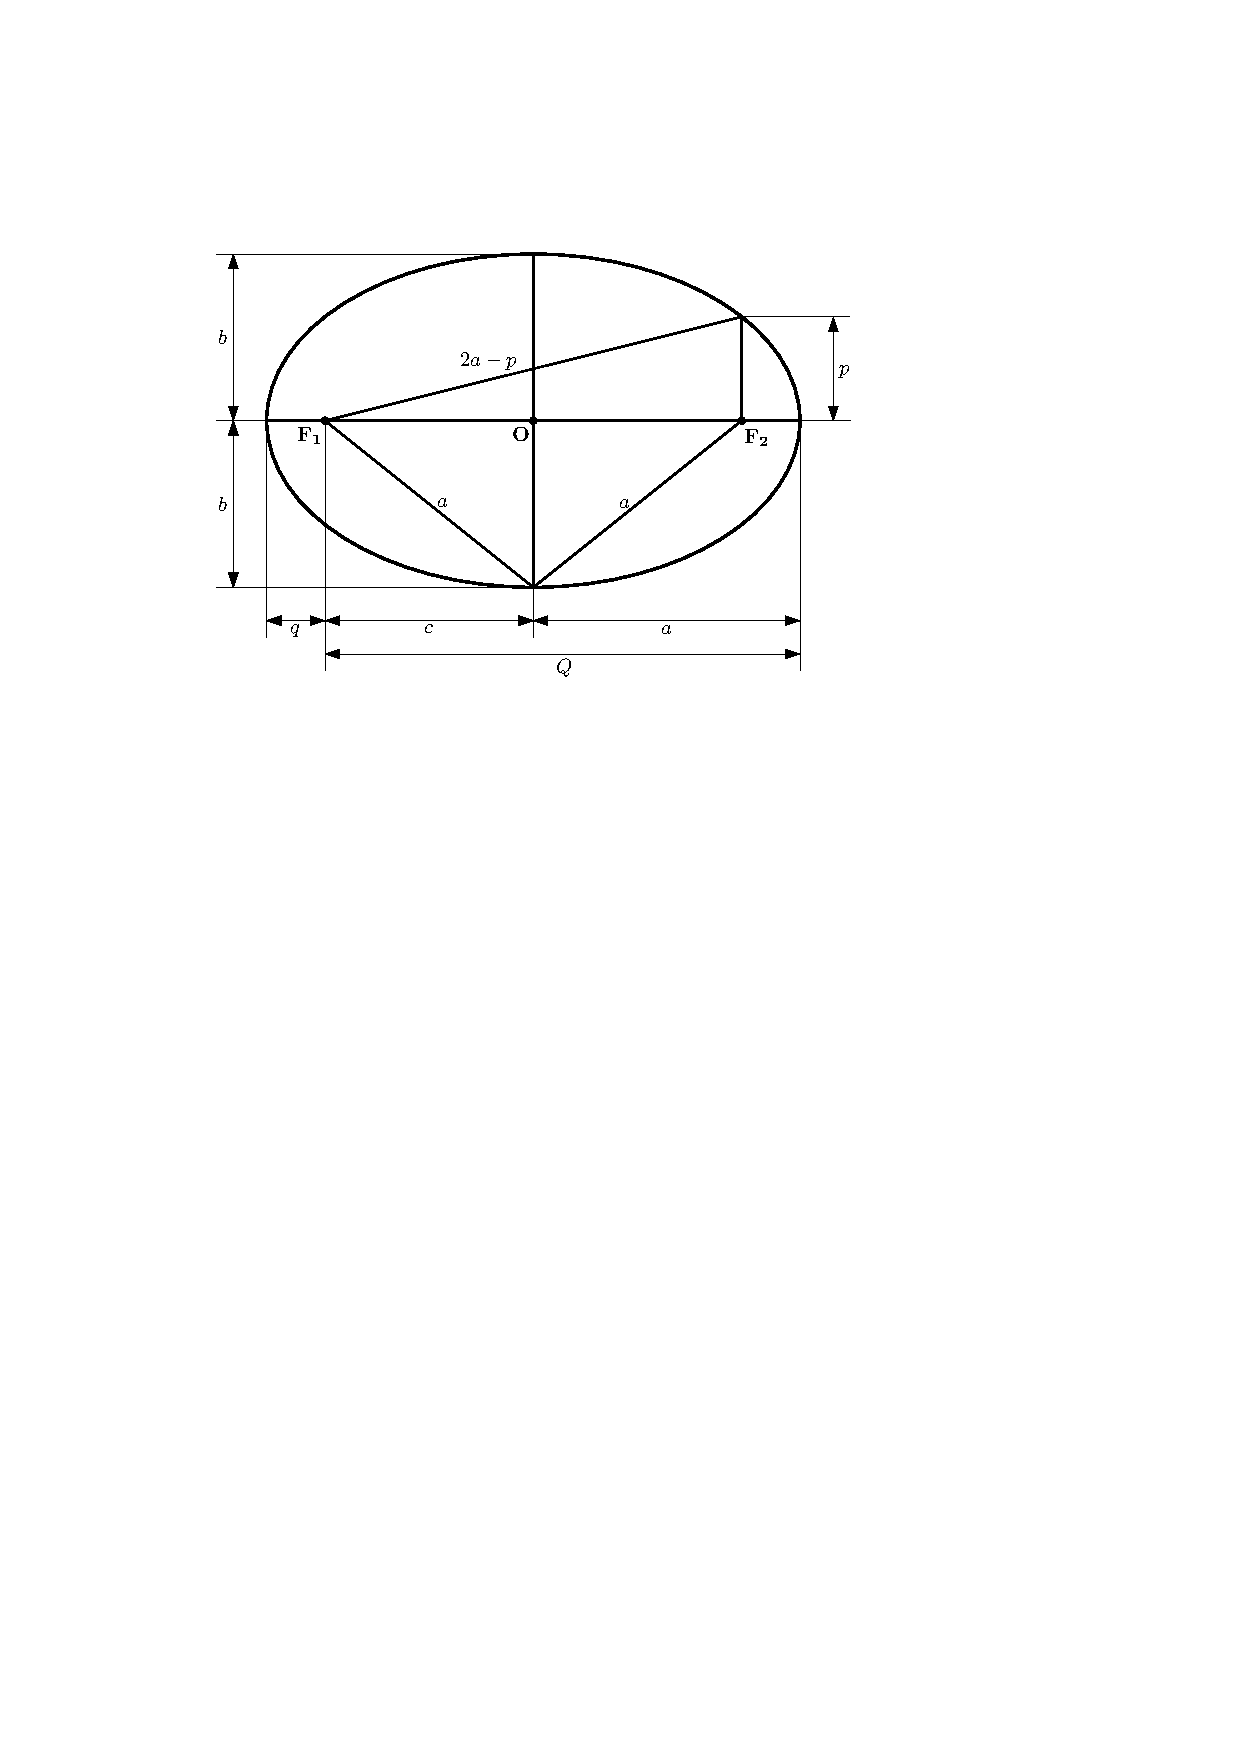
\includegraphics[width = 0.8\textwidth]{Ellips}
\caption{Эллипс}
\end{figure}

{\itshape Апоцентр} --- наиболее удаленная точка
от заданного фокуса точка эллипса. Из определения эллипса
вытекает соотношение для расстояния от фокуса до 
апоцентра ($Q$):\begin{equation}
Q = a (1 + e)
\end{equation}

{\itshape Перицентр} --- ближайшая точка
точка эллипса к заданному фокусу . Из определения эллипса
вытекает соотношение для расстояния от фокуса до 
перицетра ($q$):\begin{equation}
q = a (1 - e)
\end{equation}

{\itshape Фокальный параметр} ($p$) --- длина перпендикуляра,
проведенного из фокуса до точки пересечения с эллипсом.
Из теоремы Пифагора и определения эллипса следует 
нижеприведенная формула для расчета его длины. 
\begin{equation}
p = a(1 - e^2)
\end{equation}

{\itshape Площадь эллипса} ($S$) --- площадь части 
плоскости, ограниченной эллипсом. Выражение для площади 
эллипса можно находить интегрированием по полярному углу, 
используя уравнение эллипса в полярных координатах или 
пользуясь свойством аффинного преобразования сжатия из 
выражения площади окружности с радиусом $a$:
\begin{equation}
S=\pi ab
\end{equation}

%Радиус кривизны дуги эллипса в зависимости от расстояния 
%$x$ от фокуса:
%\begin{equation}
%R=\frac{(2ax-x^2)^{3/2}}{ab}
%\end{equation}
%\begin{center}
%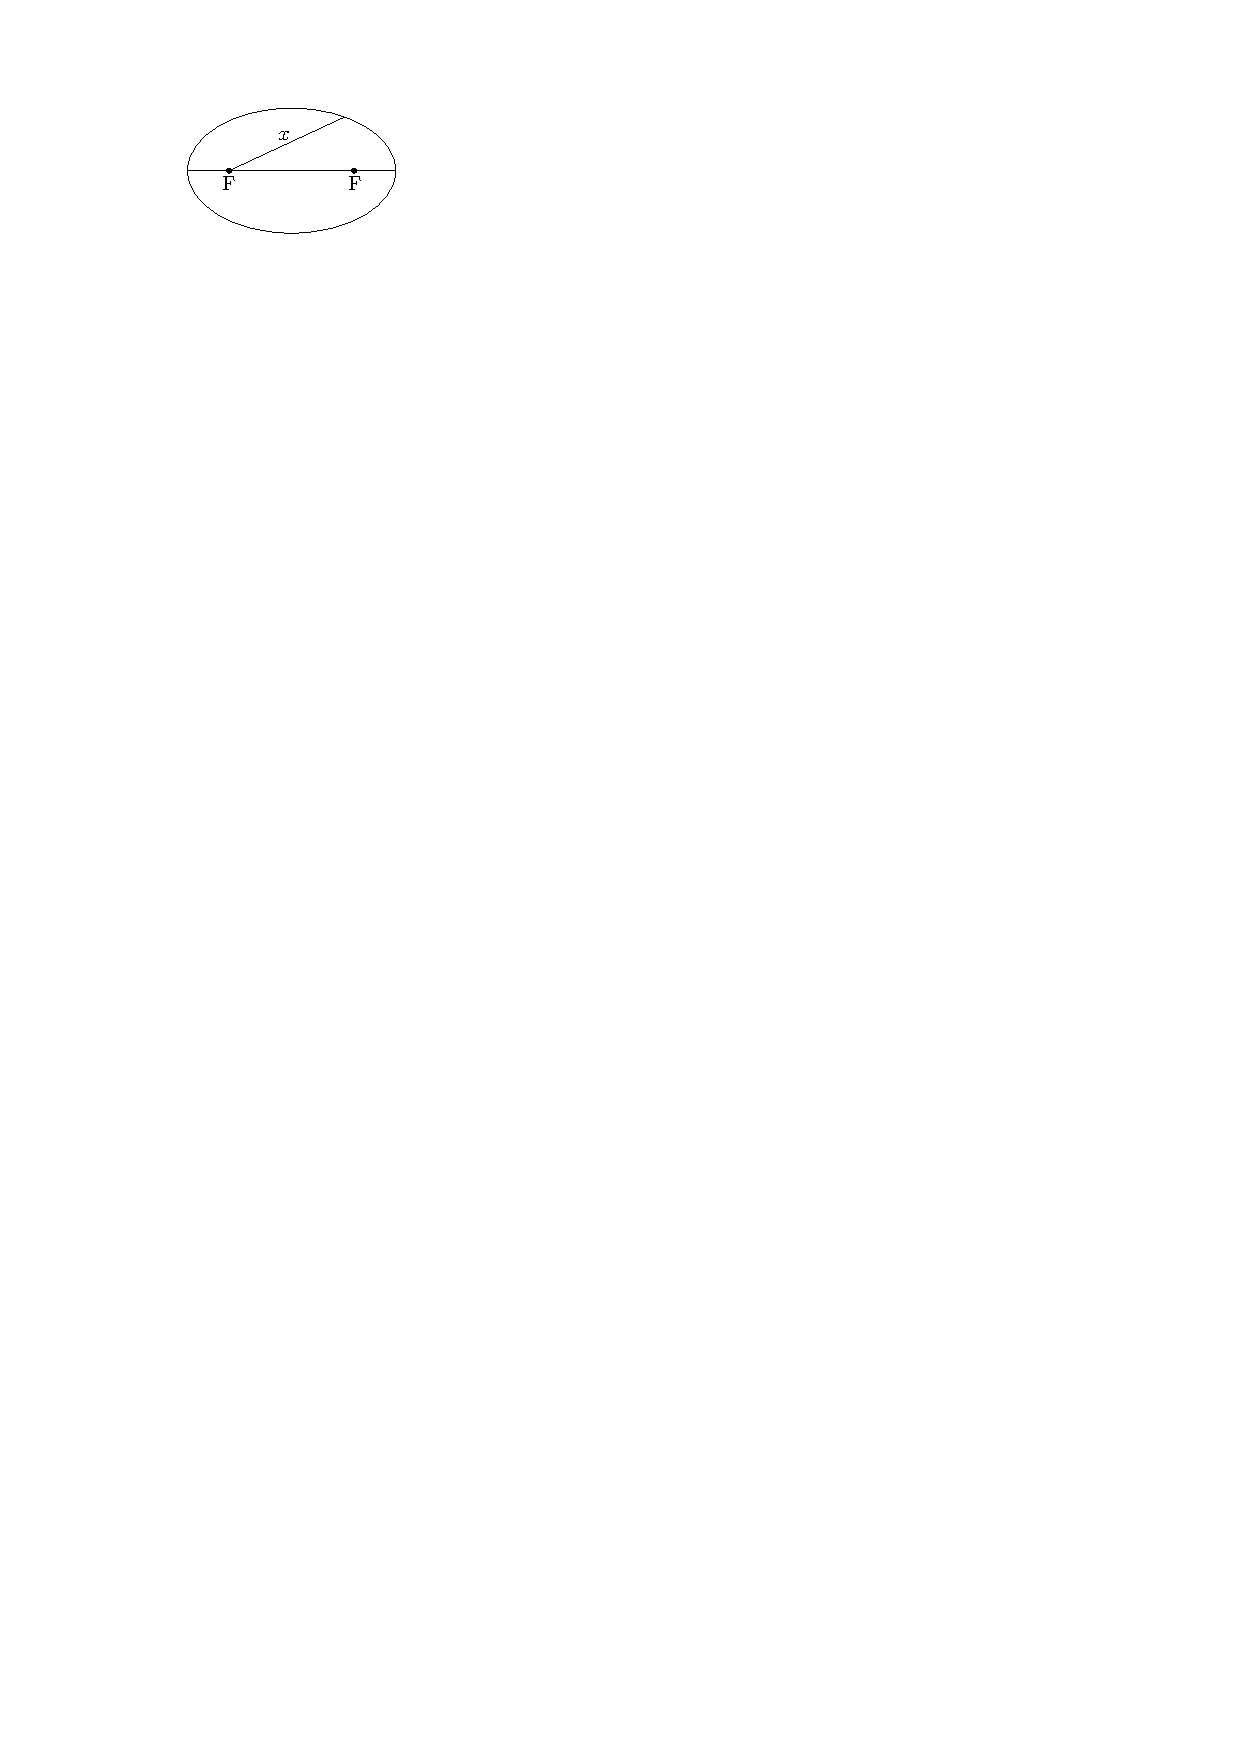
\includegraphics[width = 0.3\textwidth]{rad-curv}
%\begin{figure}[!h]
%\caption{К вычислению радиуса кривизны эллипса}
%\end{figure}
%\end{center}

{\itshape Уравнение эллипса} в декартовых координатах 
представляет собой уравнение замкнутой кривой второго 
порядка, канонический вид которого имеет следующий вид:
\begin{equation}
\frac{x^2}{a^2}+\frac{y^2}{b^2}=1
\end{equation}

Его можно представить параметрическом виде:\begin{equation}
\left\{\begin{aligned}[lcl]
&x=a\cos t\\
&y=b\sin t\\
\end{aligned}
\right.
\end{equation}
где параметр $t \in [0, \, 2\pi)$.

В полярных координатах уравнение принимает следующий вид:
\begin{equation}
r=\frac{p}{1\pm e\cos\phi}
\end{equation} 
где $\varphi$ --- {\itshape истинная аномалия} --- угол 
{\sffamily перицентр -- фокус -- заданная точка}, 
отсчитываемый в сторону движения по эллипсу. При 
положительном знаке перед $e$ второй фокус эллипса будет 
находится в точке $(0, \, 2c)$, а при отрицательном --- в 
точке $(\pi, \, 2c)$.\\

Кроме этого, эллипс обладает важным {\itshape оптическим 
свойством}, которе можно сформулировать так:
$$
\text{\begin{minipage}[]{0.4\textwidth}
	Свет от источника в одном из фокусов, 
	отражается эллипсом так, что отражённые лучи пересекаются 
	во втором фокусе.
\end{minipage}} \quad \Longleftrightarrow  \quad 
\text{\begin{minipage}{0.4\textwidth}
	Касательная к эллипсу в заданной точке образует с 
	фокальными радиусами в данной точке равные острые углы.
\end{minipage}}
$$






 
